% -----------------------------------------------------------------------------
% centriMembSolver — Theory, Implementation and Usage Guide
%
% This document serves as a combined user and developer guide for
% ``centriMembSolver``, an OpenFOAM® based solver developed for rotating
% membrane systems.  It is written in the spirit of the RheoTool
% documentation: concise, technically precise and self‑contained.  The
% solver couples hydrodynamics, solute transport, centrifugal
% acceleration and osmotic effects across semi‑permeable boundaries.  A
% robust semi‑implicit algorithm for the Coriolis term is described in
% detail along with the membrane boundary conditions and overall solver
% architecture.

\documentclass[11pt,a4paper]{article}

% ------------------------- Packages and settings -------------------------
\usepackage[utf8]{inputenc}
\usepackage[T1]{fontenc}
\usepackage{amsmath,amssymb}
\usepackage{siunitx}
\usepackage{graphicx}
\usepackage{booktabs}
\usepackage{tikz}
\usepackage{hyperref}
\usepackage{geometry}
\usepackage{caption}
\usepackage{subcaption}

\geometry{margin=25mm}
\setlength{\parindent}{0pt}
\setlength{\parskip}{1ex plus 0.5ex minus 0.2ex}
\hypersetup{colorlinks=true,linkcolor=blue,urlcolor=blue,citecolor=blue}

% ------------------------ Title and meta information ------------------------
\title{\bfseries centriMembSolver — Theory, Implementation and Usage Guide\\[1ex]
\large A combined user and developer manual for rotating membrane simulations}
\author{SmartFreez R\&D Group\\University of Lisbon, 2025}
\date{\today}

\begin{document}

\maketitle

\begin{abstract}
\noindent
\texttt{centriMembSolver} is a finite–volume solver for coupled solvent and
solute transport through rotating membranes.  Developed as part of the
SmartFreez research programme, it extends \texttt{pimpleFoam} to include
semi‑permeable membrane boundary conditions, concentration dependent
viscosity and a numerically robust semi‑implicit treatment of the Coriolis
force.  This guide documents the underlying theory, the
implementation of membrane flux models and the overall solver
architecture.  A worked example, \emph{rotatingSlit}, is included to
illustrate setup and post–processing.  The document is intended both for
end–users running membrane simulations and for developers wishing to
extend the solver to new flux laws or multi–physics couplings.
\end{abstract}

\tableofcontents

% ===========================================================================
\section{Introduction}

Rotating membrane systems combine fluid flow, solute transport and
selective separation in a centrifugal field.  Applications range from
ultra–scale–down (USD) process development, where small membrane coupons
are rotated at high speed to emulate industrial centrifugation, to
cryogenic membrane filtration in biotechnology.  In these systems a
pressure gradient drives solvent through a semi–permeable barrier while a
concentration difference induces osmotic counterflow.  Rotation adds
centrifugal and Coriolis effects that modify the hydrodynamics and
solute distribution.

\texttt{centriMembSolver} was developed to provide an open and
customisable platform for simulating such coupled phenomena.  Built on
OpenFOAM® v2506, the solver solves the incompressible Navier–Stokes
equations with source terms for rotation, a scalar transport equation
for solute concentration and custom patch fields to model membrane
fluxes.  A key feature of the implementation is a \emph{semi–implicit
Coriolis integration} which retains numerical stability at high
rotational speeds.  In addition, the membrane boundary conditions
implement well established flux laws—Spiegler–Kedem, constant flux and
target average flux for the solvent, and intrinsic rejection, solute
permeability or observed rejection for the solute.  Diagnostic
quantities such as observed rejection and concentration polarisation are
computed automatically.

The following sections present the governing equations (including
viscous and osmotic effects), derive the robust Coriolis algorithm,
detail the boundary conditions, describe the solver structure and
illustrate usage through a case study.  Developer notes at the end
provide guidance on extending the code and best practice for stable
simulations.

% ===========================================================================


\section{Theory and Governing Equations}

\subsection{Hydrodynamics}

In a non-inertial reference frame rotating with angular velocity
\(\boldsymbol{\Omega}\), the incompressible Navier–Stokes equations read
\begin{equation}
	\nabla\cdot\mathbf{U} = 0,\qquad
	\rho \frac{\partial\mathbf{U}}{\partial t} + \rho\,\nabla\cdot(\mathbf{U}\mathbf{U})
	= -\nabla p + \nabla\cdot(\mu_{\mathrm{eff}}\nabla\mathbf{U})
	+ \rho\,\mathbf{f}_{\mathrm{rot}},
\end{equation}
where \(\mathbf{U}\) is the velocity, \(p\) the kinematic pressure
(\(p=p_{\mathrm{phys}}/\rho\)), and the effective viscosity
\(\mu_{\mathrm{eff}} = \rho(\nu + \nu_t)\) includes molecular and—if
selected—turbulent viscosity.

The rotational body force \(\mathbf{f}_{\mathrm{rot}}\) contains
centrifugal and Coriolis terms
\begin{equation}
	\mathbf{f}_{\mathrm{rot}}
	= \boldsymbol{\Omega}\times(\boldsymbol{\Omega}\times\mathbf{r})
	- 2\,\boldsymbol{\Omega}\times\mathbf{U},
\end{equation}
with \(\mathbf{r}\) the position vector in the rotating frame.
Pressure–velocity coupling is handled by the PIMPLE algorithm, as
implemented in \texttt{UEqn.H} and \texttt{pEqn.H}.







\subsubsection{Modified pressure, hydrostatic potential and Boussinesq buoyancy}

Rotating membrane devices exhibit very large hydrostatic pressure
gradients, dominated by centrifugal effects. The physical pressure
\(p\) may increase by several bars over a few centimetres of radius,
while the dynamic variations induced by fluid motion are much smaller.
If \(p\) is solved directly, the linear systems become ill–conditioned
and the convergence of the PIMPLE algorithm deteriorates.

To avoid this, \texttt{centriMembSolver} follows the standard OpenFOAM
strategy and works with three auxiliary fields:

\begin{itemize}
	\item \texttt{p\_rgh}: modified (dynamic) pressure
	\item \texttt{gh}: hydrostatic potential per unit mass
	\item \texttt{rhok}: dimensionless density ratio
\end{itemize}

The solver only solves for the dynamic component \texttt{p\_rgh}; the
hydrostatic contribution is treated analytically via \texttt{gh} and
\texttt{rhok}.

\paragraph{Boussinesq density field}

Under the Boussinesq approximation, the density depends weakly on
solute concentration but remains close to a reference value \(\rho_0\):
\begin{equation}
	\rho(\boldsymbol{x}) = \rho_0\,\rho_k(\boldsymbol{x}),
	\qquad
	|\rho_k - 1| \ll 1,
\end{equation}
where the code field \texttt{rhok} corresponds to the scalar
\(\rho_k\). The flow is treated as incompressible,
\begin{equation}
	\nabla\cdot\boldsymbol{U} = 0,
	\qquad
	\frac{\partial \rho}{\partial t} = 0,
\end{equation}
but density variations (\(\rho_k \neq 1\)) still generate buoyancy forces.

\paragraph{Effective acceleration in the rotating frame}

Let \(\boldsymbol{x}\) denote the position vector in the rotating frame
and \(\boldsymbol{x}_0\) the axis of rotation (from
\texttt{SRFProperties}). A fluid particle at rest in this frame is
subject to gravity and centrifugal acceleration:
\begin{equation}
	\boldsymbol{a}_{\mathrm{eff}}(\boldsymbol{x})
	=
	\boldsymbol{g}
	-
	\boldsymbol{\Omega}\times
	\bigl(
	\boldsymbol{\Omega}\times(\boldsymbol{x}-\boldsymbol{x}_0)
	\bigr),
	\label{eq:a_eff}
\end{equation}
where \(\boldsymbol{g}\) is the gravitational acceleration and
\(\boldsymbol{\Omega}\) the angular velocity vector.

The Coriolis term \(-2\,\boldsymbol{\Omega}\times\boldsymbol{U}\) is
non–conservative and is therefore \emph{not} included in
\(\boldsymbol{a}_{\mathrm{eff}}\).

\paragraph{Hydrostatic potential \texttt{gh}}

The key point is that the effective acceleration \(\boldsymbol{a}_{\rm eff}\)
in \eqref{eq:a_eff} is conservative: it can be written as the gradient
of a scalar potential per unit mass. OpenFOAM stores this potential in
the field \texttt{gh}, defined so that
\begin{equation}
	\nabla (\mathrm{gh}) = \boldsymbol{a}_{\mathrm{eff}}.
\end{equation}

A convenient explicit expression is
\begin{equation}
	\mathrm{gh}(\boldsymbol{x})
	=
	\boldsymbol{g}\cdot(\boldsymbol{x}-\boldsymbol{x}_{\mathrm{ref}})
	+ \frac{1}{2}
	\left|
	\boldsymbol{\Omega}\times(\boldsymbol{x}-\boldsymbol{x}_0)
	\right|^2
	- \mathrm{gh}_{\mathrm{ref}},
	\label{eq:gh_def}
\end{equation}
where \(\boldsymbol{x}_{\mathrm{ref}}\) is a reference point and
\(\mathrm{gh}_{\mathrm{ref}}\) is a constant offset. This offset does not
affect the physics, since only gradients of \(\mathrm{gh}\) enter the
equations.

\medskip
\noindent
\textbf{Physical meaning.}
\(\mathrm{gh}\) is the hydrostatic potential per unit mass, combining
gravitational and centrifugal contributions. Surfaces of constant
\(\mathrm{gh}\) correspond to equilibrium surfaces of a fluid at rest
under gravity and rotation.

\paragraph{Modified pressure \(p_{\mathrm{rgh}}\)}

In the solver, the physical pressure is reconstructed from the three
fields \texttt{p\_rgh}, \texttt{gh} and \texttt{rhok} as
\begin{equation}
	p(\boldsymbol{x})
	=
	\rho_0\bigl(
	p_{\mathrm{rgh}}(\boldsymbol{x})
	+ \rho_k(\boldsymbol{x})\,\mathrm{gh}(\boldsymbol{x})
	\bigr)
	+ p_{\mathrm{ref}},
	\label{eq:p_reconstruct}
\end{equation}
where \(p_{\mathrm{rgh}}\) corresponds to the OpenFOAM field
\texttt{p\_rgh} and \(p_{\mathrm{ref}}\) is a constant reference pressure.

Neglecting the constant \(p_{\mathrm{ref}}/\rho_0\), this can be
rearranged as
\begin{equation}
	p_{\mathrm{rgh}}
	=
	\frac{p}{\rho_0}
	- \rho_k\,\mathrm{gh}.
	\label{eq:p_rgh_def}
\end{equation}

Thus \(p_{\mathrm{rgh}}\) represents the \emph{dynamic} part of the
pressure: the large hydrostatic background is removed and only the
smaller fluctuations are handled by the linear solver.

\paragraph{Momentum equation in \(p_{\mathrm{rgh}}\) form}

The incompressible rotating–frame Navier–Stokes equation under
Boussinesq can be written as
\begin{equation}
	\rho_0\rho_k
	\left(
	\frac{\partial \boldsymbol{U}}{\partial t}
	+ \boldsymbol{U}\cdot\nabla\boldsymbol{U}
	\right)
	=
	-\nabla p
	+ \nabla\cdot\bigl(\mu_{\mathrm{eff}}\nabla\boldsymbol{U}\bigr)
	+ \rho_0\rho_k\,\boldsymbol{a}_{\mathrm{eff}}
	- 2\rho_0\rho_k\,\boldsymbol{\Omega}\times\boldsymbol{U}.
	\label{eq:NS_raw}
\end{equation}

\paragraph{Step-by-step transformation to the \(p_{\mathrm{rgh}}\)-based form}

Using the definition \eqref{eq:p_rgh_def},
\[
p
= \rho_0\left(p_{\mathrm{rgh}} + \rho_k\,\mathrm{gh}\right),
\]
the pressure gradient becomes
\begin{align}
	-\nabla p
	&= -\rho_0 \nabla\!\left(p_{\mathrm{rgh}} + \rho_k\,\mathrm{gh}\right)
	\nonumber\\
	&= -\rho_0\nabla p_{\mathrm{rgh}}
	-\rho_0\nabla(\rho_k\,\mathrm{gh}).
\end{align}
Applying the product rule,
\begin{equation}
	\nabla(\rho_k\,\mathrm{gh})
	=
	\mathrm{gh}\,\nabla\rho_k
	+
	\rho_k\,\nabla(\mathrm{gh})
	=
	\mathrm{gh}\,\nabla\rho_k
	+
	\rho_k\,\boldsymbol{a}_{\mathrm{eff}},
\end{equation}
where we used \(\nabla(\mathrm{gh}) = \boldsymbol{a}_{\mathrm{eff}}\).
Thus
\begin{equation}
	-\nabla p
	=
	-\rho_0\nabla p_{\mathrm{rgh}}
	-\rho_0\,\mathrm{gh}\,\nabla\rho_k
	-\rho_0\rho_k\,\boldsymbol{a}_{\mathrm{eff}}.
	\label{eq:pressure_expanded}
\end{equation}

Substituting \eqref{eq:pressure_expanded} into \eqref{eq:NS_raw} and
cancelling the \(\rho_0\rho_k\,\boldsymbol{a}_{\mathrm{eff}}\) terms on
both sides yields
\begin{equation}
	\rho_0
	\left(
	\frac{\partial \boldsymbol{U}}{\partial t}
	+ \boldsymbol{U}\cdot\nabla\boldsymbol{U}
	\right)
	=
	- \rho_0\nabla p_{\mathrm{rgh}}
	- \rho_0\,\mathrm{gh}\,\nabla\rho_k
	+ \nabla\cdot\bigl(\mu_{\mathrm{eff}}\nabla\boldsymbol{U}\bigr)
	- 2\rho_0\rho_k\,\boldsymbol{\Omega}\times\boldsymbol{U}.
	\label{eq:NS_prgh_rho0}
\end{equation}

Since \(\rho_0\) is constant, we can divide the entire equation by
\(\rho_0\) to obtain the canonical form used in the solver:
\begin{equation}
	\rho_k
	\left(
	\frac{\partial \boldsymbol{U}}{\partial t}
	+ \boldsymbol{U}\cdot\nabla\boldsymbol{U}
	\right)
	=
	- \nabla p_{\mathrm{rgh}}
	- \mathrm{gh}\,\nabla\rho_k
	+
	\frac{1}{\rho_0}\nabla\cdot\bigl(\mu_{\mathrm{eff}}\nabla\boldsymbol{U}\bigr)
	- 2\rho_k\,\boldsymbol{\Omega}\times\boldsymbol{U}.
	\label{eq:NS_prgh}
\end{equation}

The hydrostatic load has disappeared from the unknown pressure
(\(p_{\mathrm{rgh}}\)), and only the term proportional to
\(\nabla\rho_k\) remains as a Boussinesq buoyancy force.

\paragraph{Discrete buoyancy term in \texttt{centriMembSolver}}

The continuous term
\(-\,\mathrm{gh}\,\nabla\rho_k\)
is discretised in OpenFOAM using face–based gradients:
\begin{equation}
	-\,\mathrm{gh}\,\nabla\rho_k
	\quad\Longrightarrow\quad
	-\,\mathrm{gh}_f\,\mathrm{snGrad}(\rho_k),
\end{equation}
where \(\mathrm{gh}_f\) is the potential field interpolated to the
faces, and \(\mathrm{snGrad}(\rho_k)\) is the surface–normal gradient of
\(\rho_k\). In the actual code this appears as
\begin{verbatim}
	- ghf * fvc::snGrad(rhok)
\end{verbatim}
inside the reconstruction of the right–hand side of the momentum
equation.

\paragraph{Summary and physical interpretation}

\begin{itemize}
	\item \(\mathrm{gh}\) is the hydrostatic potential per unit mass:
	it combines gravitational and centrifugal contributions and is
	computed from geometry, \(\boldsymbol{g}\) and \(\boldsymbol{\Omega}\).
	\item \(\rho_k\) (field \texttt{rhok}) encodes density variations
	relative to \(\rho_0\) and is responsible for Boussinesq
	buoyancy.
	\item \(p_{\mathrm{rgh}}\) (field \texttt{p\_rgh}) is the pressure
	variable actually solved by PIMPLE; its gradients are much
	smaller than those of the physical pressure \(p\).
	\item The buoyancy force appears as
	\(-\,\mathrm{gh}\,\nabla\rho_k\), discretised in the code
	as \texttt{- ghf*fvc::snGrad(rhok)}.
	\item The physical pressure used for membrane transport and
	post–processing is reconstructed via \eqref{eq:p_reconstruct}.
\end{itemize}

\subsubsection{Turbulence modelling}

Although centrifugal membrane filtration can operate in laminar,
transitional or weakly turbulent regimes, \texttt{centriMembSolver}
allows the user to select any turbulence model available in the
\texttt{RASModel} hierarchy of OpenFOAM.  The model is instantiated via
the usual run-time selection mechanism in \texttt{createFields.H}:
\begin{equation}
	\nu_{\mathrm{eff}}
	= \nu + \nu_t(\mathbf{U}, k, \varepsilon, \dots).
\end{equation}

Typical configurations rely on:
\begin{itemize}
	\item direct laminar modelling (\texttt{simulationType laminar;})
	\item one–equation eddy–viscosity models such as Spalart–Allmaras
	\item two–equation models such as standard or low-Re \(k{-}\varepsilon\)
	~and \(k{-}\omega\)
\end{itemize}
with parameters defined in \texttt{constant/turbulenceProperties}.
Turbulent mass transport uses an eddy diffusivity
\(D_t = \nu_t / \mathrm{Sc}_t\), where \(\mathrm{Sc}_t\) is the turbulent
Schmidt number.

\subsubsection{Concentration-dependent viscosity}

Many cryoprotectant solutions exhibit a strong dependence of viscosity
on the solute concentration \(C_A\).  \texttt{centriMembSolver}
incorporates a polynomial parameterisation:
\begin{equation}
	\nu(C_A) = \nu_0 + \nu_1 C_A + \nu_2 C_A^2 + \cdots,
\end{equation}
with coefficients \(\nu_0,\nu_1,\nu_2\) set in
\texttt{transportProperties}.  A clipping operator prevents unphysical
values at high concentrations.


\subsection{Solute transport}

The solute concentration field obeys an advection–diffusion equation:
\begin{equation}
	\frac{\partial C_A}{\partial t}
	+ \nabla\cdot(C_A\mathbf{U})
	= \nabla\cdot(D_{\mathrm{eff}}\nabla C_A),
\end{equation}
with \(D_{\mathrm{eff}} = D_{AB} + D_t\), where \(D_{AB}\) is the
molecular diffusivity and \(D_t\) the turbulent contribution (if
enabled).  Membrane boundary conditions impose fluxes as described in
\S\ref{sec:bc-solute}.

\subsection{Osmotic pressure and flux definitions}

Transmembrane transport is driven by hydrostatic
\(\Delta p = p_f - p_p\) and osmotic \(\Delta\pi = \pi(C_{A,f}) -
\pi(C_{A,p})\) differences.  Osmotic pressure uses a virial expansion:
\begin{equation}
	\pi(C_A) = \sum_{k=1}^{N} a_k C_A^k,
\end{equation}
reducing to the van ’t Hoff law for \(a_1=RT\).

The solvent flux \(J_v\) [m/s] is formulated using the
Spiegler–Kedem relation:
\begin{equation}
	J_v = A\bigl(\Delta p - \sigma\Delta\pi\bigr),
	\label{eq:jv-s-k}
\end{equation}
where \(A\) is the hydraulic permeability and \(\sigma\) the reflection
coefficient.  Solute flux \(J_s\) [kg/(m$^2$s)] is
\begin{equation}
	J_s = (1-\sigma)J_vC_w + B(C_w - C_p),
	\label{eq:js-s-k}
\end{equation}
with intrinsic solute permeability \(B\) and wall/permeate
concentrations \(C_w\) and \(C_p\).



\section{Coriolis Term and Its Numerical Treatment in the Momentum Equation}
\label{sec:coriolis}

Rotating flows are formulated in a reference frame with angular velocity
\(\boldsymbol{\Omega}\). The Coriolis acceleration acting on a fluid
parcel is
\begin{equation}
	\mathbf{f}_{C} = -2\,\boldsymbol{\Omega} \times \mathbf{U}.
\end{equation}

In \texttt{centriMembSolver}, the Coriolis operator is evaluated at the
temporal midpoint in each time step,
\begin{equation}
	\mathbf{U}^{n+1/2}
	\approx \frac{1}{2}
	\left( \mathbf{U}^{n} + \mathbf{U}^{n+1} \right),
	\label{eq:midpointU}
\end{equation}
using the updated velocity available in the current PIMPLE iteration.
This ensures a centered-in-time discretization of the Coriolis
acceleration,
\begin{equation}
	\mathbf{f}_{C}^{n+1/2}
	= -2 \, \boldsymbol{\Omega}
	\times \mathbf{U}^{n+1/2},
\end{equation}
preserving the skew–symmetry of the operator and therefore the
discrete kinetic-energy balance of the rotational term.

\subsection{Momentum equation}

The momentum equation, solved within the PIMPLE loop, is
\begin{equation}
	\mathcal{A}(\mathbf{U})
	-
	\left(
	-2\,\boldsymbol{\Omega}\times \mathbf{U}^{n+1/2}
	\right)
	=
	\text{RHS},
\end{equation}
implemented as:
\begin{verbatim}
	Umid = 0.5*(U.oldTime() + U);
	coriolisSrc = -2.0*(omega ^ Umid);
	
	fvVectorMatrix UEqn
	(
	fvm::ddt(U)
	+ fvm::div(phi,U)
	+ turbulence->divDevReff(U)
	- coriolisSrc
	==
	fvOptions(U)
	);
\end{verbatim}

\subsection{Coupling strategy}

Because the mid-point velocity uses the updated value of \(\mathbf{U}\)
from the current corrector, the Coriolis term evolves consistently with
the pressure–velocity coupling. For DNS configurations, the
\texttt{momentumPredictor} is disabled to avoid spurious Courant number
excursions induced by the predictor in strongly rotating flows. A
single outer corrector per time step is sufficient due to the small
time steps imposed by the CFL restriction.

\subsection{Summary}

The Coriolis acceleration in \texttt{centriMembSolver} is discretized
at the temporal midpoint and updated at every PIMPLE iteration. This
yields a robust, energy-consistent and publication-grade formulation
suitable for the extreme rotational conditions characteristic of
centrifugal membrane systems.

\section{Membrane Boundary Conditions}

Membrane patches couple the feed region to the permeate side by
imposing fluxes of solvent and solute according to physical models.
\texttt{centriMembSolver} implements two specialised patch field
classes: \texttt{membraneSolventFluxFvPatchVectorField} for the
velocity and \texttt{membraneSoluteFluxFvPatchScalarField} for the
concentration.  The feed side of the membrane is the patch
corresponding to the field values; permeate side conditions are
either fixed (for constant pressure/concentration) or inferred from
the flux law.

\subsection{Solvent flux boundary (\texttt{U})}
The solvent flux condition determines the normal component of
\(\mathbf{U}\) at the membrane.  Three models are provided:

\paragraph{Spiegler–Kedem model.}
Implements Eq.~\eqref{eq:jv-s-k}.  Dictionary entries include the
hydraulic permeability \texttt{Ah}, the reflection coefficient
\texttt{sigma}, virial coefficients \texttt{virialCoeffs} for the
osmotic pressure and an optional permeate pressure \texttt{pPermConst}
and concentration \texttt{CAPermConst}.  The example below sets
\texttt{Ah = 0.5e-11}, \texttt{sigma = 1.0}, \texttt{virialCoeffs
 (0 0)} for a van ’t Hoff law and assumes permeate pressure zero:

\begin{verbatim}
membraneA
{
    type    membraneSolventFlux;
    model   SpieglerKedem;
    Ah      0.5e-11;        // [m/(Pa s)]
    sigma   1.0;            // [-]
    virialCoeffs (0);       // a1 = RT, a2 = 0
    pPermConst 0;           // [Pa]
    CAPermConst 0;          // [kg/m3]
    value  uniform (0 0 0);
}
\end{verbatim}

\paragraph{Constant flux model.}
Prescribes a uniform solvent flux \(J_v\) independent of driving
forces.  Use the key \texttt{Jv} to set the flux magnitude (in
\si{m/s}).  This model is useful for benchmarking or when the
membrane permeability is unknown.

\paragraph{Target average flux model.}
Tunes an effective permeability \(A_\mathrm{eff}\) such that the area–
averaged flux matches a target \texttt{JvAverage}.  Driving forces are
still proportional to \(\Delta p - \sigma \Delta \pi\) as in the
Spiegler–Kedem model, but \(A_\mathrm{eff}\) is updated each time
step within user–specified bounds \texttt{AhMin} and \texttt{AhMax}.
This is particularly useful for calibrating models against measured
permeabilities.

\paragraph{Diagnostics.}
For each membrane patch the solver writes the instantaneous and
time–windowed area–average of \(J_v\).  If window averaging is
enabled (\texttt{windowAverage true}), the time scale \texttt{Twindow}
sets the averaging duration.  The internal field \texttt{Jv} is
available for further post–processing.

\subsection{Solute flux boundary (\texttt{CA})}
\label{sec:bc-solute}
The solute boundary condition couples the solute transport to the
solvent flux.  Three models are available:

\paragraph{Intrinsic rejection model.}
Assumes that a fraction \(R_\mathrm{int}\) of the solute is rejected at
the membrane such that the permeate concentration is
\(C_p = (1 - R_\mathrm{int})\,C_w\).  The wall concentration \(C_w\)
follows a film balance
\begin{equation}
  k\,(C_w - C_i) = R_\mathrm{int}\,J_v\,C_w,
\end{equation}
where \(k\) is the mass transfer coefficient and \(C_i\) the bulk
concentration adjacent to the membrane.  Solute flux is simply
\(J_s=J_v C_p\).  Dictionary entries are \texttt{model
 intrinsicRejection}, \texttt{Rint} and the reference concentration
\texttt{CAb} used for diagnostics.

\paragraph{Solute permeability model.}
Implements Eq.~\eqref{eq:js-s-k} with a solute permeability \(B\).  If
\texttt{sigma} is specified it overrides the reflection coefficient
from the solvent BC; otherwise \(\sigma\) is inherited.  This model
reduces to a solution–diffusion model when \(\sigma=0\).

\paragraph{Observed rejection model.}
Targets a desired observed rejection \(R_\mathrm{obs}\) defined by
\begin{equation}
  R_\mathrm{obs} = 1 - \frac{\langle J_v C_p \rangle}{\langle J_v \rangle\,C_{A,b}},
\end{equation}
where \(\langle\cdot\rangle\) denotes an area average and \(C_{A,b}\)
is the bulk reference concentration.  The solver iteratively
determines an intrinsic rejection \(R_\mathrm{int}\) such that the
observed rejection matches the target within a specified tolerance.
Controls include \texttt{Robs} (target), \texttt{RintMin},
\texttt{RintMax}, \texttt{tol} and \texttt{maxIter}.  This is
particularly useful when matching experimental data for rejection.

\paragraph{Diagnostics.}
Per–face fluxes \(J_s\), \(J_v\) and permeate concentration \(C_p\) are
exposed to the solver via the patch fields \texttt{Js}, \texttt{Jv}
and \texttt{CAp}, and are written to the file
\texttt{postProcessing/membraneSoluteFlux/<patch>/Rint\_vs\_time.dat}.
The solver also outputs the observed rejection and concentration
polarisation factor \(\Gamma=(C_w - C_{A,b})/C_{A,b}\) for post–
processing.

\subsection{Membrane patch dictionaries}

Tables~\ref{tab:membrane-solvent} and~\ref{tab:membrane-solute}
summarise the principal dictionary entries for solvent and solute
boundary conditions.  Most values default to physically reasonable
numbers; only those shown as required must be provided.

\begin{table}[h]
  \centering
  \caption{Summary of membrane solvent flux boundary entries.}
  \label{tab:membrane-solvent}
  \begin{tabular}{@{}llp{8cm}@{}}
    \toprule
    Key & Units & Description\\
    \midrule
    \texttt{model} & – & \texttt{SpieglerKedem}, \texttt{constantFlux} or \texttt{targetAverageFlux}\\
    \texttt{Ah} & \si{m/(Pa\,s)} & Hydraulic permeability for Spiegler–Kedem\\
    \texttt{sigma} & – & Reflection coefficient \(\sigma\); defaults to 1\\
    \texttt{virialCoeffs} & – & List \((a_1,a_2,\dots)\) for osmotic pressure\\
    \texttt{Jv} & \si{m/s} & Constant flux magnitude (constantFlux model)\\
    \texttt{JvAverage} & \si{m/s} & Target area–average flux (targetAverageFlux)\\
    \texttt{AhMin}, \texttt{AhMax} & \si{m/(Pa\,s)} & Limits on tuned permeability\\
    \texttt{pPermConst}, \texttt{CAPermConst} & – & Fixed permeate side pressure/concentration\\
    \texttt{windowAverage}, \texttt{Twindow} & – & Enable and set window for time–averaged output\\
    \bottomrule
  \end{tabular}
\end{table}

\begin{table}[h]
  \centering
  \caption{Summary of membrane solute flux boundary entries.}
  \label{tab:membrane-solute}
  \begin{tabular}{@{}llp{8cm}@{}}
    \toprule
    Key & Units & Description\\
    \midrule
    \texttt{model} & – & \texttt{intrinsicRejection}, \texttt{solutePermeability} or \texttt{observedRejection}\\
    \texttt{Rint} & – & Intrinsic rejection coefficient (intrinsicRejection)\\
    \texttt{B} & \si{m/s} & Solute permeability (solutePermeability)\\
    \texttt{sigma} & – & Optional reflection coefficient (overrides solvent BC)\\
    \texttt{Robs} & – & Target observed rejection (observedRejection)\\
    \texttt{CAb} & \si{kg/m^3} & Reference bulk concentration for diagnostics\\
    \texttt{RintMin}, \texttt{RintMax} & – & Bounds for inverse rejection search\\
    \texttt{tol}, \texttt{maxIter} & – & Tolerance and maximum iterations for secant/bisection\\
    \texttt{UName} & – & Name of velocity field (defaults to \texttt{U})\\
    \bottomrule
  \end{tabular}
\end{table}

% ===========================================================================


\section{Solver structure and implementation}

The \texttt{centriMembSolver} follows a PIMPLE--type pressure--velocity
coupling, extended with (i) concentration--dependent transport
properties, (ii) a rotating reference frame, and (iii) custom membrane
boundary conditions and diagnostics. The overall time loop is driven by
\texttt{runTime.run()}, and at each time step a nested PIMPLE loop
solves momentum, pressure and solute transport. Additional headers
perform pressure reconstruction and conservation monitoring before the
fields are written.

\subsection{Overall time loop and custom PIMPLE algorithm}

For readers familiar with C++, the main structure of
\texttt{centriMembSolver.C} can be summarised schematically as

\begin{verbatim}
	createTime;
	createMesh;
	createControl;              // pimpleControl
	createFields;               // U, p_rgh, CA, etc.
	membraneFields;             // Js, Jv, CAp, Gama
	updateTransportProperties;  // nu(CA), DAB(CA), rhok
	
	while (runTime.run())
	{
		// (normally: compute Courant number and time-step)
		
		++runTime;
		Info<< "Time = " << runTime.timeName() << endl;
		
		while (pimple.loop())           // outer PIMPLE loop
		{
			#include "UEqn.H"           // assemble & solve momentum
			#include "CAEqn.H"          // assemble & solve solute
			#include "updateTransportProperties.H"
			
			while (pimple.correct())    // inner pressure loop
			{
				#include "pEqn.H"
			}
			
			if (pimple.turbCorr())
			{
				turbulence->correct();
			}
		}
		
		#include "pReconstruct.H"
		#include "monitorConservation.H"
		#include "Gama.H"
		#include "forces.H"
		
		runTime.write();
		runTime.printExecutionTime(Info);
	}
\end{verbatim}

Compared with a ``standard'' OpenFOAM transient solver:

\begin{itemize}
	\item momentum \texttt{(UEqn.H)} and solute \texttt{(CAEqn.H)} are
	solved together at the beginning of each PIMPLE outer iteration;
	\item transport properties (viscosity, diffusivity, density) are
	updated \emph{inside} the PIMPLE loop via
	\texttt{updateTransportProperties.H}, so they respond
	iteratively to the current concentration field;
	\item several post--processing steps (absolute pressure, conservation,
	membrane diagnostic \(\Gamma\), body forces) are executed at the
	end of every time step.
\end{itemize}

This design makes the coupling between flow, solute transport and
membrane behaviour explicit while still using the familiar PIMPLE
machinery.

\subsection{Field creation, membrane diagnostics and transport properties}

Field creation is handled in two main headers:

\begin{itemize}
	\item \textbf{\texttt{createFields.H}} reads the primary fields
	(\texttt{U}, \texttt{p\_rgh}, \texttt{CA}, etc.) from the
	\texttt{0/} directory and the physical parameters from
	\texttt{constant/transportProperties} and
	\texttt{constant/SRFProperties}. It also constructs the
	turbulence model if required.
	
	\item \textbf{\texttt{membraneFields.H}} declares four additional
	volume fields used for membrane diagnostics:
	\texttt{Js} (solute flux), \texttt{Jv} (solvent flux),
	\texttt{CAp} (permeate concentration) and \texttt{Gama} (a
	dimensionless diagnostic \(\Gamma\)). All are created with
	\texttt{AUTO\_WRITE}, so they are automatically written at
	output times.
\end{itemize}

The header \texttt{updateTransportProperties.H} is called once before
the time loop and then at each outer PIMPLE iteration. It performs three
updates:

\begin{enumerate}
	\item \emph{Viscosity}: the laminar transport model
	\texttt{laminarTransport} is corrected using the current
	concentration field \texttt{CA}, so that the kinematic viscosity
	\(\nu(\mathrm{CA})\) follows the chosen \texttt{CAViscosity}
	model.
	
	\item \emph{Molecular diffusivity}: the scalar field \texttt{DAB} is
	updated as a function of \texttt{CA}, using a polynomial
	relation. Boundary conditions on \texttt{DAB} are corrected
	afterwards.
	
	\item \emph{Density}: a non--dimensional density field \texttt{rhok}
	is recomputed according to a Boussinesq--type law,
	\(\rho_k = 1 + \beta\,\mathrm{CA}\), and its boundary
	conditions are corrected.
\end{enumerate}

Updating these properties inside the PIMPLE loop strengthens the
coupling between momentum and solute transport: any change in
\texttt{CA} is immediately reflected in \(\nu\), \(D_{AB}\) and
\(\rho_k\).

\subsection{Momentum and pressure equations}

Inside the outer \texttt{while (pimple.loop())}:

\begin{itemize}
	\item \textbf{\texttt{UEqn.H}} assembles the transient momentum
	equation using implicit time discretisation
	(\texttt{fvm::ddt}), a convection term
	\texttt{fvm::div(phi,U)}, viscous/turbulent stresses via
	\texttt{turbulence->divDevReff(U)}, and a Coriolis source term
	\(2\rho\,\boldsymbol{\Omega}\times\mathbf{U}\) for the rotating
	frame. The equation is then solved for the velocity field
	\texttt{U}.
	
	\item \textbf{\texttt{CAEqn.H}} assembles and solves the unsteady
	advection--diffusion equation for the solute concentration
	\texttt{CA}, using a Crank--Nicolson scheme in time and a
	bounded convection scheme in space.
\end{itemize}

After these solves, \texttt{updateTransportProperties.H} is called again
to refresh \(\nu(\mathrm{CA})\), \(D_{AB}(\mathrm{CA})\) and \(\rho_k\)
based on the newly updated \texttt{CA} field.

The pressure equation is then handled in the inner loop
\texttt{while (pimple.correct())} through \texttt{pEqn.H}. This step
enforces continuity, updates \texttt{p\_rgh} (and the associated face
flux \texttt{phi}) and accounts for the rotation--induced hydrostatic
term and the specified pressure reference. When
\texttt{pimple.turbCorr()} is true, the turbulence model is also
corrected in the same outer iteration.

\subsection{Membrane boundary conditions and the \texorpdfstring{$\Gamma$}{Gamma} diagnostic}

The actual membrane physics is implemented in custom boundary condition
classes applied to \texttt{U} and \texttt{CA}. These boundary
conditions:

\begin{itemize}
	\item compute, for each membrane face, the solvent flux \(J_v\) and
	solute flux \(J_s\) according to the selected transport model
	(e.g. pressure--driven with osmotic correction);
	\item update the permeate concentration \(C_p\) and a dimensionless
	diagnostic \(\Gamma\) that characterises local solute rejection
	or concentration polarisation.
\end{itemize}

At volume level, these per--face quantities are exported into the
diagnostic fields declared in \texttt{membraneFields.H}. The header
\texttt{Gama.H} is responsible for copying the per--face \(\Gamma\)
values from the membrane solute boundary condition into the boundary of
the volume field \texttt{Gama}, so that \texttt{Gama} can be visualised
and sampled like any other \texttt{volScalarField}. For efficiency,
\texttt{Gama.H} caches the membrane patch indices and a pointer to the
\texttt{CA} field the first time it is called.

\subsection{Post-processing: pressure reconstruction, conservation and forces}

After the PIMPLE loop converges at a given time, four post--processing
headers are executed before writing:

\paragraph{\texttt{pReconstruct.H}}

The solver works internally with the modified pressure \texttt{p\_rgh}
to simplify the treatment of gravity in a rotating frame. For analysis,
it is convenient to have the absolute pressure field. The header
\texttt{pReconstruct.H} reconstructs

\[
p = (p\_\text{rgh} + \rho_k\,g\,h)\,\rho_0 + p_\text{ref},
\]

where \(\rho_0\) is a reference density and \(p_\text{ref}\) the chosen
pressure reference, and then calls \texttt{p.correctBoundaryConditions()}
to keep the boundaries consistent.

\paragraph{\texttt{monitorConservation.H}}

This header checks global solute conservation in a parallel--safe way.
It requires the fields \texttt{CA}, \texttt{U}, \texttt{Js},
\texttt{Jv}, \texttt{CAp} and the face flux \texttt{phi}; an optional
\texttt{Deff} field can be supplied to account for diffusive fluxes at
walls. It builds (or appends to) the file

\[
\texttt{postProcessing/conservation/cons.dat},
\]

writing at each output time the total solute mass in the domain, the
time derivative of that mass, the integrated inlet, outlet, membrane and
diffusive contributions, and a residual and relative error that measure
how well the discrete balance is satisfied. This file is the main tool
to verify that the coupled flow--membrane scheme is globally
conservative.

\paragraph{\texttt{Gama.H}}

As described above, \texttt{Gama.H} maps the per--face diagnostic
\(\Gamma\) from the membrane boundary condition into the volume field
\texttt{Gama}. This is done patch by patch on the membrane boundaries,
with simple consistency checks (same number of faces) to avoid copying
errors.

\paragraph{\texttt{forces.H}}

Finally, \texttt{forces.H} computes two auxiliary vector fields:

\begin{align*}
	\mathbf{a}_\mathrm{Coriolis} &= 2\,\boldsymbol{\Omega}\times\mathbf{U},
	\\
	\mathbf{a}_\mathrm{buoy} &= g\,h\,\nabla\rho_k,
\end{align*}

stored in the fields \texttt{aCoriolis} and \texttt{aBuoy}. These
fields do not influence the solution; they are provided for
post--processing and interpretation, allowing the user to visualise the
spatial structure and relative magnitude of Coriolis and buoyancy
effects in the rotating device.

At the end of this post--processing stage,
\texttt{runTime.write()} writes all \texttt{AUTO\_WRITE} fields
(\texttt{U}, \texttt{p}, \texttt{p\_rgh}, \texttt{CA}, \texttt{Js},
\texttt{Jv}, \texttt{CAp}, \texttt{Gama}, \texttt{aCoriolis},
\texttt{aBuoy}, etc.), and the solver advances to the next time level.

% ===========================================================================


\section{Case studies with \texttt{centriMembSolver}}

This section presents two example cases that illustrate how to use
\texttt{centriMembSolver}.  They are designed to be readable even for
readers who are not familiar with OpenFOAM.

In OpenFOAM, each simulation (``case'') is stored in a directory with a
standard structure:
\begin{itemize}
	\item \texttt{0/} contains the \emph{initial and boundary conditions}
	for all fields (for example velocity, pressure and concentration);
	\item \texttt{constant/} contains the \emph{physical properties}
	(for example fluid properties, solute properties, membrane
	parameters, rotation settings);
	\item \texttt{system/} contains the \emph{numerical setup}
	(mesh generation with \texttt{blockMesh}, time step controls,
	linear solvers, etc.).
\end{itemize}

To run a case, one typically:
\begin{enumerate}
	\item generates the mesh (for example with \texttt{blockMesh} or a
	helper script);
	\item runs the solver (here \texttt{centriMembSolver});
	\item inspects the results in ParaView or in text files written in
	\texttt{postProcessing/}.
\end{enumerate}

Below we describe two specific cases: a simple 2D slit
(\texttt{rotatingSlit}) and a centrifugal configuration
(\texttt{O-CFM}).

% ---------------------------------------------------------------------------
\subsection{\texttt{rotatingSlit}}

The example case \texttt{rotatingSlit} distributed with the solver
provides a simple yet instructive demonstration.  It consists of a
two-dimensional slit domain rotated about its centre.  The membrane
occupies a section of the side wall; the remaining boundaries are
inlet, outlet, symmetry and empty patches.

\subsubsection*{Geometry and mesh}

The geometry is defined by \texttt{system/blockMeshDict}.  A narrow
slit of length \SI{4}{\centi\metre} and width \SI{1}{\milli\metre} is
discretised into a structured mesh.  One boundary, named
\texttt{membraneB}, is assigned the membrane boundary conditions.  A
second boundary \texttt{membraneA} is present but disabled in this
case.  Front and back patches are declared as \texttt{empty} to
produce a two-dimensional simulation.

\subsubsection*{Initial and boundary conditions}

The inlet velocity $\mathbf{U}$ is a fixed value, typically
\SI{0.01}{m/s}, driving flow along the slit.  The initial solute
concentration is uniform (\SI{5}{kg/m^3}) and the inlet condition sets
\texttt{CAin} to a higher or lower value to induce concentration
polarisation.  The membrane on patch \texttt{membraneB} is configured
with
\begin{itemize}
	\item a target average solvent flux of \SI{3e-5}{m/s},
	\item limits \texttt{AhMin = 1e-13} and \texttt{AhMax = 1e-9},
	\item reflection coefficient $\sigma=1$, and
	\item virial coefficients
	$(7314.5\,\mathrm{Pa\,m^3\,kg^{-1}},
	8.253\,\mathrm{Pa\,m^6\,kg^{-2}})$.
\end{itemize}
On the solute side the membrane uses the intrinsic rejection model with
\texttt{Rint = 0.99} and reference concentration \texttt{CAb = 1.0}.  A
fixed–flux pressure condition ensures continuity of volumetric flow.

\subsubsection*{Running the case}

To run the example, follow these steps in the case directory:

\begin{enumerate}
	\item Compile the solver (only needed once) by executing \texttt{wmake}
	in the \texttt{solver} directory.
	\item Generate the mesh using
	\begin{verbatim}
		blockMesh
	\end{verbatim}
	\item Adjust \texttt{constant/SRFProperties} to set the rotation
	speed $\boldsymbol{\Omega}$ if desired.  The default example uses
	\texttt{rpm = 0}, but any non–zero value can be specified.
	\item Run the simulation with
	\begin{verbatim}
		centriMembSolver -case rotatingSlit > log &
	\end{verbatim}
	\item Monitor progress via the log or the files in
	\texttt{postProcessing}.  Key outputs include
	\texttt{Rint\_vs\_time.dat} (intrinsic rejection over time),
	\texttt{calibratedProperties.dat} (effective permeability for
	target average flux) and \texttt{cons.dat} (mass conservation).
\end{enumerate}

Figure~\ref{fig:rotatingSlit-results} sketches typical results: the area–
average solvent flux approaches the target \SI{3e-5}{m/s} after a
short transient; the intrinsic rejection remains close to the specified
value; and the concentration polarisation builds up at the membrane.

\begin{figure}[h]
	\centering
	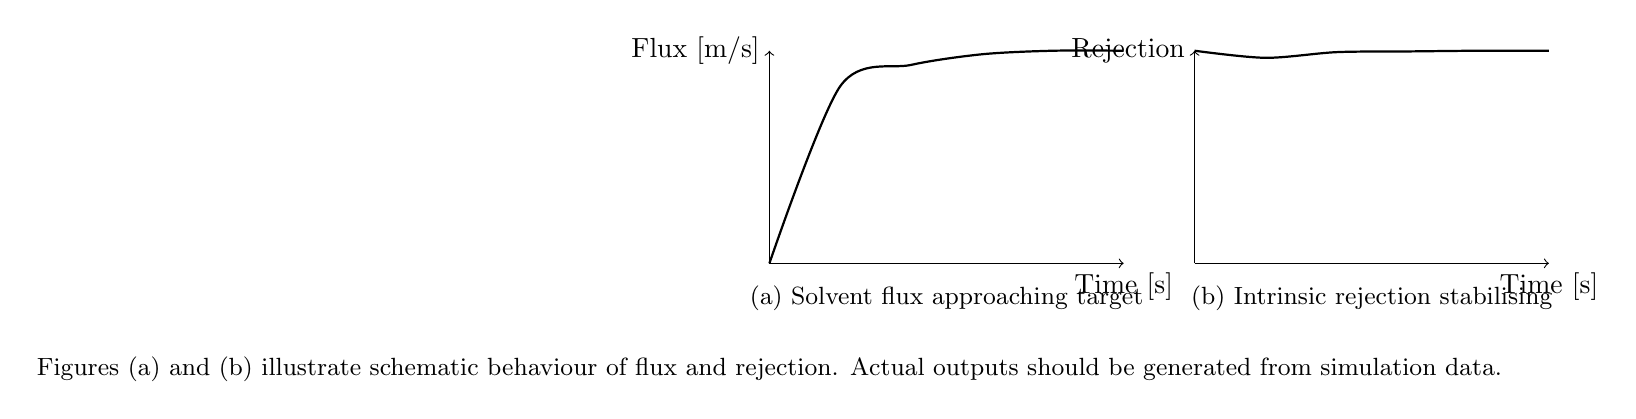
\begin{tikzpicture}[scale=0.9]
		% Axes for flux plot
		\begin{scope}
			\draw[->] (0,0) -- (5,0) node[below]{Time [s]};
			\draw[->] (0,0) -- (0,3) node[left]{Flux [m/s]};
			\draw[smooth,thick] plot coordinates{
				(0.0,0.0) (1,2.5) (2,2.8) (3,2.95) (4,3.0) (5,3.0)};
			\node at (2.5,-0.5) {\small (a) Solvent flux approaching target};
		\end{scope}
		% Axes for rejection plot
		\begin{scope}[xshift=6cm]
			\draw[->] (0,0) -- (5,0) node[below]{Time [s]};
			\draw[->] (0,0) -- (0,3) node[left]{Rejection};
			\draw[smooth,thick] plot coordinates{
				(0.0,3) (1,2.9) (2,2.98) (3,2.99) (4,3.0) (5,3.0)};
			\node at (2.5,-0.5) {\small (b) Intrinsic rejection stabilising};
		\end{scope}
		\node at (0,-1.5) {\small Figures (a) and (b) illustrate schematic behaviour
			of flux and rejection. Actual outputs should be generated from
			simulation data.};
	\end{tikzpicture}
	\caption{Qualitative results from the \texttt{rotatingSlit} example:
		(a) the area–averaged solvent flux converges to the target value
		specified in the dictionary; (b) the intrinsic rejection computed by
		the solver stabilises to the prescribed parameter.}
	\label{fig:rotatingSlit-results}
\end{figure}

% ---------------------------------------------------------------------------
\subsection{\texttt{O-CFM}}

The \texttt{O-CFM} case represents a centrifugal membrane configuration,
in which the domain rotates at a prescribed angular velocity.  Rotation
creates a radial pressure gradient that drives solvent through a
membrane located at the outer radius.  This case also demonstrates the
use of helper scripts for mesh generation and parallel execution.

\subsubsection*{Geometry and mesh}

The geometry and mesh are defined indirectly through the script
\texttt{makeMesh}, which in turn uses \texttt{system/blockMeshDict}.
The domain can be thought of as an annular sector:

\begin{itemize}
	\item an inner radius $r_\mathrm{in}$ that acts as the feed region,
	\item an outer radius $r_\mathrm{out}$ where the membrane is located,
	\item a small angular extent (sector) in the circumferential direction,
	\item front and back patches set to \texttt{empty} to obtain a 2D
	approximation.
\end{itemize}

The membrane is assigned to the outer radial wall (for example a patch
named \texttt{outerWall} in the mesh).  The mesh resolution and sector
angle are chosen to provide a compromise between accuracy and runtime.

To generate the mesh, one simply runs
\begin{verbatim}
	./makeMesh
\end{verbatim}
in the case directory.

\subsubsection*{Rotation, physics and solute properties}

Rotation is defined in \texttt{constant/SRFProperties} by specifying the
angular velocity (for example via \texttt{rpm}).  The solver then
includes the corresponding centrifugal and Coriolis terms in the
momentum equation, so that the apparent pressure increases with radius.

The solute in this case is magnesium sulphate (MgSO$_4$).  Its
properties are stored in files such as \texttt{constant/MgSO4} and
\texttt{constant/transportProperties}, which define, for example:
\begin{itemize}
	\item diffusion coefficient of MgSO$_4$ in water,
	\item solution density and viscosity as functions of concentration,
	\item parameters for the osmotic pressure model (for example virial
	coefficients).
\end{itemize}

Boundary conditions follow the typical centrifugal filtration concept:
\begin{itemize}
	\item feed is introduced near $r_\mathrm{in}$ with a specified
	velocity and solute concentration,
	\item the membrane at $r_\mathrm{out}$ imposes a controlled solvent
	flux and a given intrinsic rejection for MgSO$_4$,
	\item the pressure field adjusts to balance centrifugal forcing,
	membrane permeation and any imposed outlet or recycle
	conditions.
\end{itemize}

\subsubsection*{Running the case}

The \texttt{O-CFM} case is prepared to run in parallel.  A convenience
script \texttt{runCaseParallel} handles decomposition, solver execution
and reconstruction.  From the case directory one can execute:
\begin{verbatim}
	./makeMesh
	./runCaseParallel
\end{verbatim}

Internally, this typically performs the following steps:
\begin{enumerate}
	\item decomposes the domain into subdomains (for example using
	\texttt{decomposePar}),
	\item calls \texttt{mpirun} or an equivalent launcher with
	\texttt{centriMembSolver},
	\item reconstructs the final fields for visualisation.
\end{enumerate}

If desired, the case can also be run in serial by skipping the
decomposition and calling \texttt{centriMembSolver} directly.

\subsubsection*{Typical results and diagnostics}

In this centrifugal configuration the rotation produces:
\begin{itemize}
	\item an increasing pressure profile from $r_\mathrm{in}$ to
	$r_\mathrm{out}$,
	\item enhanced solvent flux through the membrane at the outer radius,
	\item strong radial concentration gradients and concentration
	polarisation at the membrane,
	\item significant shear near the membrane, which tends to limit the
	thickness of the concentration boundary layer.
\end{itemize}

As with the \texttt{rotatingSlit} case, the solver can write diagnostic
files in \texttt{postProcessing/} to monitor, for example:
\begin{itemize}
	\item global mass conservation (similar to \texttt{cons.dat}),
	\item time evolution of average membrane flux,
	\item average intrinsic rejection of MgSO$_4$.
\end{itemize}

Together, the \texttt{rotatingSlit} and \texttt{O-CFM} cases provide a
pair of simple but representative examples: a planar slit for basic
membrane calibration and a rotating annulus for centrifugal membrane
operation.
% ===========================================================================

\section{Developer Notes and Best Practices}

\subsection{Extending boundary conditions}

New flux models can be added by subclassing the existing patch field
classes.  To create a new solvent flux law, derive from
\texttt{membraneSolventFluxFvPatchVectorField}, add a new enumerated
identifier in the \texttt{Model} enum and implement the logic in
\texttt{updateCoeffs()}.  Register the class with the runtime
selection table using \texttt{addToRunTimeSelectionTable}.  Follow a
similar procedure for solute flux models.

Ensure that any new model reads user–specified parameters from the
dictionary and writes meaningful diagnostics.  When coupling new
physics (e.g.~temperature or multiple solutes), extend the field lists
in \texttt{createFields.H} and update the transport properties
accordingly.

\subsection{Stability and time stepping}

Although the semi–implicit Coriolis integration relaxes the time–step
constraint on rotation, the convective CFL condition still applies.
Maintain the Courant number below 1 near the membrane.  When using
target average flux, choose \texttt{AhMin} and \texttt{AhMax} such
that the calibration remains stable; too wide a range may lead to
oscillatory behaviour.  For observed rejection, choose tight tolerances
\texttt{tol} and ensure that the target lies within the physically
realistic range defined by \texttt{RintMin} and \texttt{RintMax}.

\subsection{Parallel consistency}

The boundary conditions and diagnostics use parallel reductions to
ensure consistent results across processors.  Nevertheless, for
complex geometries or very fine meshes it is advisable to use
\texttt{redistributePar} when decomposing the domain so that membrane
patches are not split across processors.  The conservation monitor
provides a quick check on mass balances across processor boundaries.

\subsection{Further development}

Possible extensions include: coupling multiple solutes with different
permeabilities; including heat transfer and temperature–dependent
permeability; implementing steric hindrance models; coupling with
chemical reactions or variable membrane area.  The modular design of
\texttt{centriMembSolver} facilitates such developments.  To implement
temperature effects, for instance, one would introduce a temperature
field, modify the viscosity and osmotic pressure models to depend on
temperature and augment the boundary condition dictionaries with
temperature–dependent coefficients.

% ===========================================================================
\section{References}

\begin{enumerate}
	\item Spiegler, K. S. \& Kedem, O. (1966). Thermodynamics of hyperfiltration (reverse osmosis): criteria for efficient membranes. \emph{Desalination}, 1, 311–326.
	\item Wu, J. J. (2019). On the application of the Spiegler–Kedem model to forward osmosis. \emph{BMC Chemical Engineering}, 1, 15.  (Discusses how the S–K model allows deviation from ideal semi–permeability.)
	\item Cayley, A. (1846). A theorem on skew–symmetric matrices.  Summarised in the definition of the Cayley transform: for a skew–symmetric matrix \(A\), the map \((I - A)(I + A)^{-1}\) yields an orthogonal matrix.
	\item Coriolis force formula.  The acceleration of a mass in a rotating frame includes a term \(-2\,\boldsymbol{\Omega}\times\mathbf{v}\) acting orthogonal to the velocity.
\end{enumerate}

\appendix

\section{Appendix A: Implementing Boundary Conditions in OpenFOAM}

This appendix is intended for students who want to understand how the
membrane boundary conditions are implemented inside OpenFOAM, and for
those who may wish to extend or modify them.

% -------------------------------------------------------------------
\subsection{B.1 Boundary conditions as C++ objects}

Every boundary condition in OpenFOAM is a small C++ class derived from:

\begin{itemize}
	\item \texttt{fvPatchField} (generic base),
	\item \texttt{fvPatchScalarField} (scalar fields),
	\item \texttt{fvPatchVectorField} (vector fields).
\end{itemize}

Each patch entry in \texttt{0/U}, \texttt{0/p} or \texttt{0/CA}
creates one of these C++ objects at run time.

A custom BC must define:

\begin{itemize}
	\item a \textbf{TypeName} so OpenFOAM can select it,
	\item constructors to read user parameters,
	\item an \textbf{updateCoeffs()} method to apply the physics.
\end{itemize}

The file structure is typically:

\begin{verbatim}
	MyBC/
	MyBCFvPatchField.H
	MyBCFvPatchField.C
\end{verbatim}

Compiled into a dynamic library with \texttt{wmake libso}.

% -------------------------------------------------------------------
\subsection{B.2 What constructors do (and must NOT do)}

Constructors:

\begin{itemize}
	\item read parameters from the dictionary,
	\item initialise private member data,
	\item check dimensions and required fields.
\end{itemize}

They must \emph{not} impose the boundary condition.  
This is the role of \texttt{updateCoeffs()}.

% -------------------------------------------------------------------
\subsection{B.3 The updateCoeffs() method}

\texttt{updateCoeffs()} is the core of every BC. It is called whenever
OpenFOAM assembles the matrix for the equation being solved.

Its responsibilities:

\begin{enumerate}
	\item Guard against double updates with \texttt{if (updated()) return;} 
	\item Read internal values (e.g.\ $C_i$) from the adjacent cells.
	\item Compute the required boundary physics (e.g.\ $C_w$, $J_s$, $C_p$).
	\item Set the mixed condition via:
	\begin{verbatim}
		valueFraction()[f] = alpha;
		refValue()[f] = Cref;
		refGrad()[f]  = gradient;
	\end{verbatim}
	\item Call the base-class update with:
	\begin{verbatim}
		mixedFvPatchScalarField::updateCoeffs();
	\end{verbatim}
\end{enumerate}

For the solute membrane BC, this method contains the entire membrane
transport model; the solver itself does not handle membrane physics.

% -------------------------------------------------------------------
\subsection{B.4 Accessing geometry and fields}

Useful geometry functions inside a BC:

\begin{itemize}
	\item \texttt{patch().Sf()} : face area vectors,
	\item \texttt{patch().nf()} : face normals,
	\item \texttt{patch().magSf()} : magnitudes of areas,
	\item \texttt{deltaCoeffs()} : $1/\Delta x$ across the boundary.
\end{itemize}

Useful to read fields:

\begin{itemize}
	\item \texttt{this->patchInternalField()} : internal cell values,
	\item \texttt{db().lookupObject} : access other fields (e.g.\ \texttt{Jv}).
\end{itemize}

% -------------------------------------------------------------------
\subsection{B.5 Using custom boundary conditions}

After compiling your BC:

\begin{enumerate}
	\item Add the library name to \texttt{system/controlDict}:
	\begin{verbatim}
		libs ("libmembraneBCs.so");
	\end{verbatim}
	
	\item Specify the BC in the field file:
	\begin{verbatim}
		membrane
		{
			type membraneSoluteFlux;
			CAp CAp;
			Jv  Jv;
			Js  Js;
		}
	\end{verbatim}
	
	\item Run the solver — the BC is applied automatically.
\end{enumerate}

% -------------------------------------------------------------------
\subsection{B.6 Debugging and good practice}

\begin{itemize}
	\item Insert \texttt{Info <<} messages inside \texttt{updateCoeffs()}.
	\item Always ensure consistent units (OpenFOAM checks dimensions).
	\item To diagnose conservation, print $J_s$, $J_v$, $C_p$ each iteration.
	\item For parallel runs, use \texttt{Pstream::reduce()} to sum fluxes.
\end{itemize}

This appendix should provide enough structure for students to navigate
and extend the membrane boundary conditions within OpenFOAM.


\end{document}